\documentclass[]{informeutn}

\usepackage{siunitx}
\usepackage{icomma}
\usepackage[backend=bibtex, style=alphabetic, sorting=ynt]{biblatex}
\addbibresource{fuentes.bib}

\usepackage{subcaption}
\usepackage{listings}
\usepackage{pgfplots}
\usepackage{pdfpages}
\pgfplotsset{compat=1.18}
\usepgfplotslibrary{groupplots}
\graphicspath{{images/}{figures/}{pictures/}{./}}

\lstdefinestyle{ltspice}{
  backgroundcolor=\color{gray!10},
  basicstyle=\ttfamily\small,
  keywordstyle=\color{blue},
  frame=single,
  breaklines=true,
  captionpos=b
}

% Datos de la carátula
\materia{Electrónica Aplicada II}
\titulo{Fuentes de Alimentación Lineales}
\subtitulo{Regulador Integrado con Elevador de Corriente y Protección de Sobrecarga -- Consigna 5}
\comision{4R2}
\autores{
    Gil, Ignacio - 401891\\
    Grasso, Gaston - 401892\\
    Palombo, Franco - 401910\\
    Prieto, Angelo - 401012
}
\fecha{\today}

\begin{document}
  \maketitle
  \tableofcontents
  \setcounter{page}{1}
  \thispagestyle{plain}

  \chapter{Introducción}
\label{sec.c5:introduccion}

En esta actividad evaluativa correspondiente a la Unidad Temática 6 (Fuentes de Alimentación) se aborda el
cálculo, diseño y verificación experimental por simulación de una fuente de alimentación lineal
regulada con protección contra sobrecargas, en cumplimiento de los requerimientos fijados para la Consigna 5 del
Grupo 5.

\section{Especificaciones de diseño}
\label{sec.c5:especificaciones}

La consigna establece las siguientes condiciones operativas para el circuito:
\begin{itemize}
    \item Tensión de salida regulada: $V_{out} = \SI{12}{\volt}$ continua.
    \item Corriente máxima a plena carga: $I_{Lmax} = \SI{3}{\ampere}$.
    \item Corriente mínima de carga: $I_{Lmin} = \SI{100}{\milli\ampere}$.
    \item Componente regulador base: regulador lineal integrado de tres terminales LM7812 en encapsulado metálico TO-3.
    \item Protección: incorporación obligatoria de una etapa limitadora de sobrecarga y cortocircuito.
    \item Evaluación de desempeño: determinación de la totalidad de los factores de calidad de la fuente.
\end{itemize}

\section{Justificación de la topología seleccionada}
\label{sec.c5:topologia}

El circuito integrado LM7812 presenta una capacidad máxima de corriente nominal de salida de $\SI{1}{\ampere}$
(con un límite de disparo típico interno de $\SI{1.5}{\ampere}$ a $\SI{2.2}{\ampere}$). Dado que la carga
especificada demanda hasta $\SI{3}{\ampere}$, el integrado resulta insuficiente por sí solo para abastecer la
demanda continua sin ingresar en protección térmica o sobrecorriente interna.

Para superar esta restricción, adoptamos la configuración de \emph{elevador de corriente con transistor de paso
exterior y limitador de sobrecarga}, correspondiente a la Figura 6-67 del material teórico de la cátedra
\cite{gonzalez_fuentes3}. En este circuito, un transistor de potencia PNP ($Q_1$) conduce la mayor parte de la
corriente que excede la capacidad del regulador, mientras que un segundo transistor discreto ($Q_2$) junto a un resistor
de sensado ($R_{sc}$) forman un lazo de realimentación negativa para limitar rígidamente la corriente máxima
en caso de falla o cortocircuito franco en la salida.

  \chapter{Diseño y Cálculo Analítico}
\label{sec.c5:diseno_teorico}

\section{Selección de componentes activos}
\label{sec.c5:seleccion_activos}

Para la implementación del circuito se seleccionaron los siguientes dispositivos:
\begin{enumerate}
    \item \textbf{Regulador Integrado LM7812:} Regulador lineal positivo fijo de tres terminales. De acuerdo a la
    consigna, se adopta la versión en encapsulado metálico TO-3 (sufijo K), caracterizado por una resistencia
    térmica juntura-carcasa reducida ($\theta_{jc} \approx \SI{4}{\celsius/\watt}$ frente a los
    $\SI{5}{\celsius/\watt}$ del encapsulado plástico TO-220), lo que optimiza la transferencia de calor hacia el
    disipador común \cite{ti_lm78xx}.
    \item \textbf{Transistor de paso de potencia $Q_1$ (MJ2955):} Se seleccionó el transistor PNP de potencia
    MJ2955, complementario del 2N3055, provisto en encapsulado hermético TO-3. Admite una corriente continua de
    colector de hasta $\SI{15}{\ampere}$, una tensión colector-emisor máxima $V_{CEO} = \SI{60}{\volt}$ y una
    potencia máxima disipable $P_D = \SI{150}{\watt}$ a $T_C = \SI{25}{\celsius}$ \cite{onsemi_mj2955}.
    \item \textbf{Transistor sensor de sobrecarga $Q_2$ (BC557B):} Transistor bipolar PNP de pequeña señal en
    encapsulado TO-92 ($V_{CEO} = \SI{45}{\volt}$, $I_{Cmax} = \SI{100}{\milli\ampere}$, $h_{FE} \approx 200$--$450$).
    Su función es monitorear la caída sobre el resistor sensor y actuar sobre la base de $Q_1$.
\end{enumerate}

\section{Tensión de entrada no regulada $V_{in}$}
\label{sec.c5:vin}

El regulador LM7812 exige una tensión diferencial mínima entre entrada y salida ($V_{drop}$) de entre
$\SI{2}{\volt}$ y $\SI{2.5}{\volt}$ para sostener la regulación interna en su zona activa. A esta caída debe
sumarse la tensión en el resistor exterior de disparo $R_{ext}$ ($\approx \SI{0.7}{\volt}$). En consecuencia:
\begin{align*}
    V_{in(min)} &\ge V_{out} + V_{drop} + V_{Rext} \\
    V_{in(min)} &\ge \SI{12}{\volt} + \SI{2.5}{\volt} + \SI{0.7}{\volt} = \SI{15.2}{\volt}
\end{align*}
Adoptamos como tensión de entrada nominal continua $V_{in} = \SI{18}{\volt}$. Esta elección proporciona un margen
de seguridad dinámico de casi $\SI{3}{\volt}$ sobre el límite de dropout, garantizando que variaciones de línea
del $\pm 10\%$ ($16.2\text{ V} \le V_{in} \le 19.8\text{ V}$) no provoquen abandono de regulación.

\section{Cálculo de resistores del elevador y protección}
\label{sec.c5:calculo_resistores}

\subsection{Resistor de disparo del transistor de paso ($R_{ext}$ / $R_2$)}
El resistor $R_{ext}$ conecta el riel de entrada no regulado con la entrada del integrado y la base de $Q_1$. A bajas
corrientes de carga, el transistor $Q_1$ permanece cortado y la totalidad de la corriente circula por el LM7812.
Para que $Q_1$ comience a conducir cuando la corriente del regulador alcance un umbral seguro
$I_{reg(th)} \approx \SI{580}{\milli\ampere}$, se dimensiona:
\begin{equation}
    R_{ext} = \frac{V_{BE(Q1)}}{I_{reg(th)}} = \frac{\SI{0.7}{\volt}}{\SI{0.58}{\ampere}} \approx \SI{1.2}{\ohm}
    \label{eq.c5:rext}
\end{equation}
Se adopta el valor normalizado comercial $R_2 = \SI{1.2}{\ohm}$.

\subsection{Resistor sensor de corriente de sobrecarga ($R_{sc}$ / $R_1$)}
El resistor $R_{sc}$ se intercala en serie con el emisor de $Q_1$. A plena carga nominal ($I_L = \SI{3}{\ampere}$), la
corriente se reparte entregando $Q_1$ aproximadamente $\SI{1.8}{\ampere}$ y el regulador $\SI{1.2}{\ampere}$.
La protección de sobrecarga debe dispararse cuando la corriente del transistor exterior supere un margen seguro,
fijado en $I_{ext(max)} \approx \SI{2.6}{\ampere}$ \cite{gonzalez_fuentes3}:
\begin{equation}
    R_{sc} = \frac{V_{BE(Q2)}}{I_{ext(max)}} = \frac{\SI{0.7}{\volt}}{\SI{2.6}{\ampere}} = \SI{0.269}{\ohm}
    \label{eq.c5:rsc}
\end{equation}
Se adopta el valor comercial estándar de potencia $R_1 = \SI{0.27}{\ohm}$ (resistor de alambre cementado o metal
film de $\SI{5}{\watt}$). Con este valor, la corriente máxima teórica de colector de $Q_1$ queda fijada en:
\begin{equation}
    I_{c1(max)} = \frac{V_{BE(Q2)}}{R_{sc}} = \frac{\SI{0.7}{\volt}}{\SI{0.27}{\ohm}} = \SI{2.59}{\ampere}
    \label{eq.c5:ic1max}
\end{equation}

\section{Filtros capacitivos de desacoplo y estabilidad}
\label{sec.c5:capacitores}

Siguiendo las recomendaciones de aplicación del fabricante \cite{ti_lm78xx} y de la cátedra
\cite{gonzalez_fuentes2}:
\begin{itemize}
    \item $C_1 = \SI{0.33}{\micro\farad}$ (disco cerámico): conectado entre el pin IN del LM7812 y masa, atenúa
    efectos inductivos de línea y previene autooscilaciones parásitas de alta frecuencia.
    \item $C_2 = \SI{0.1}{\micro\farad}$ (disco cerámico): colocado en paralelo inmediato a la salida OUT del
    LM7812, garantiza el margen de fase del lazo de amplificación de error interno.
    \item $C_3 = \SI{100}{\micro\farad}$ (electrolítico de aluminio, $\SI{25}{\volt}$): reservorio de baja
    frecuencia para absorber transitorios abruptos de demanda de carga.
\end{itemize}

El circuito esquemático completo diseñado se presenta en la figura~\ref{fig.c5:esquematico}.

\begin{figure}[!ht]
    \centering
    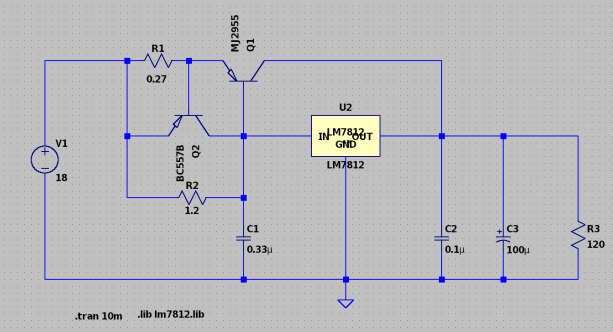
\includegraphics[width=0.88\textwidth]{sch_ltspice.png}
    \caption{Circuito esquemático completo de la fuente regulada con elevador de corriente y limitador de sobrecarga.}
    \label{fig.c5:esquematico}
\end{figure}

  \chapter{Simulación y Análisis de Sobrecarga}
\label{sec.c5:simulacion}

\section{Metodología experimental en LTspice}
\label{sec.c5:metodologia}

Para validar el circuito se utilizó los modelos SPICE del LM7812 y del TIP42C
proporcionado por los respectivos fabricantes.

Para evaluar el comportamiento de la fuente tanto en régimen normal de carga
como ante condiciones de sobrecarga y cortocircuito, se implementó en LTspice un
barrido paramétrico del resistor de carga ($R_L$) barriendo entre
$\SI{0.5}{\ohm}$ y $\SI{4.0}{\ohm}$ mediante un análisis transitorio en régimen
permanente.

\section{Resultados experimentales de sobrecarga}
\label{sec.c5:resultados_sobrecarga}

En la tabla~\ref{tab.c5:sobrecarga} se consolidan las variables eléctricas y térmicas registradas en régimen
permanente para cada escalón de carga.

\begin{table}[!ht]
\centering
\caption{Valores eléctricos y de disipación térmica en función de la resistencia de carga $R_L$.}
\label{tab.c5:sobrecarga}
\begin{tabular}{ccccccccccc}
\hline
$R_L$ & $V_{out}$ & $I_L$ & $I_C(Q_1)$ & $I_{out}(7812)$ & $V_{Rsh}$ & $I_C(Q_2)$ & $V_{CE(Q1)}$ & $P_D(Q_1)$ & $P_D(7812)$ \\
$[\si{\ohm}]$ & $[\si{\volt}]$ & $[\si{\ampere}]$ & $[\si{\ampere}]$ & $[\si{\ampere}]$ & $[\si{\volt}]$ & $[\si{\milli\ampere}]$ & $[\si{\volt}]$ & $[\si{\watt}]$ & $[\si{\watt}]$ \\
\hline
$4.0$ & $12.00$ & $3.00$ & $2.07$ & $0.93$ & $0.701$ & $141.03$  & $5.30$  & $11.04$ & $4.14$ \\
$3.5$ & $12.00$ & $3.43$ & $2.21$ & $1.22$ & $0.747$ & $397.83$  & $5.25$  & $11.68$ & $5.33$ \\
$3.0$ & $12.00$ & $4.00$ & $2.36$ & $1.64$ & $0.794$ & $787.94$  & $5.21$  & $12.35$ & $7.06$ \\
$2.5$ & $11.99$ & $4.80$ & $2.55$ & $2.25$ & $0.854$ & $1355.28$ & $5.15$  & $13.19$ & $9.49$ \\
$2.0$ & $10.59$ & $5.30$ & $2.66$ & $2.63$ & $0.890$ & $1712.24$ & $6.52$  & $17.44$ & $14.63$ \\
$1.5$ & $6.37$  & $4.24$ & $2.42$ & $1.82$ & $0.813$ & $960.51$  & $10.82$ & $26.28$ & $18.00$ \\
$1.0$ & $3.95$  & $3.95$ & $2.35$ & $1.59$ & $0.790$ & $750.38$  & $13.26$ & $31.27$ & $19.65$ \\
$0.5$ & $1.88$  & $3.77$ & $2.31$ & $1.46$ & $0.776$ & $625.48$  & $15.34$ & $35.48$ & $20.99$ \\
\hline
\end{tabular}
\end{table}

\begin{figure}[!ht]
    \centering
    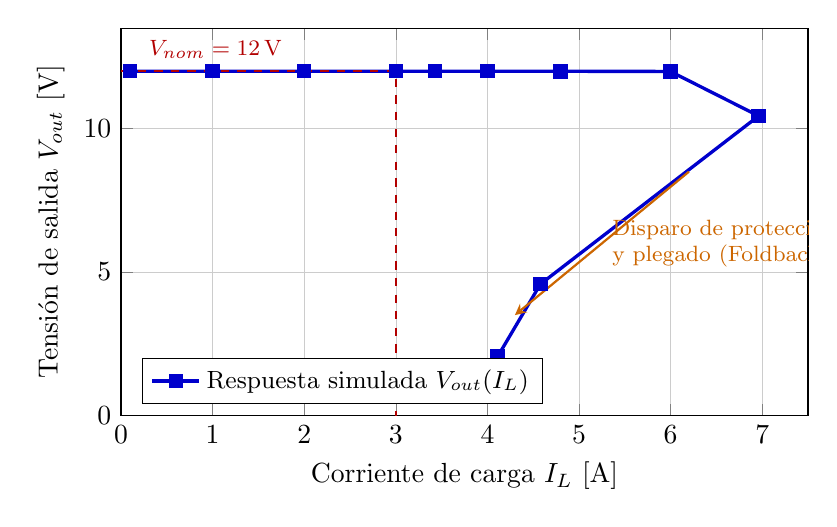
\begin{tikzpicture}
\begin{axis}[
    width=0.85\textwidth,
    height=6.5cm,
    xlabel={Corriente de carga $I_L$ [\si{\ampere}]},
    ylabel={Tensión de salida $V_{out}$ [\si{\volt}]},
    grid=both,
    grid style={line width=.1pt, draw=gray!20},
    major grid style={line width=.2pt, draw=gray!40},
    xmin=0, xmax=7.5,
    ymin=0, ymax=13.5,
    legend pos=south west,
    legend style={font=\small}
]

% Curva de salida Vo vs IL (comportamiento de tension constante y foldback)
\addplot[
    color=blue!80!black,
    mark=square*,
    mark size=2pt,
    line width=1.2pt
] coordinates {
    (0.100, 12.002)
    (1.000, 12.000)
    (2.000, 12.000)
    (3.000, 11.999)
    (3.428, 11.999)
    (4.000, 11.999)
    (4.799, 11.998)
    (5.997, 11.994)
    (6.961, 10.442)
    (4.578, 4.578)
    (4.112, 2.056)
};
\addlegendentry{Respuesta simulada $V_{out}(I_L)$}

% Linea de referencia nominal
\addplot[dashed, color=red!70!black, line width=0.8pt] coordinates {
    (0, 12) (3, 12) (3, 0)
};
\node[anchor=south west, text=red!70!black, font=\footnotesize] at (axis cs: 0.2, 12.1) {$V_{nom} = \SI{12}{\volt}$};
\node[anchor=south, text=red!70!black, font=\footnotesize] at (axis cs: 3.0, 0.2) {$I_{Lmax} = \SI{3}{\ampere}$};

% Anotacion de zona de foldback / corto
\draw[->, >=stealth, line width=0.8pt, color=orange!80!black] 
    (axis cs: 6.2, 8.5) -- (axis cs: 4.3, 3.5) 
    node[midway, right, font=\footnotesize, align=left] {Disparo de protección\\y plegado (Foldback)};

\end{axis}
\end{tikzpicture}

    \caption{Curva característica de salida $V_{out}$ en función de la corriente de carga $I_L$.}
    \label{fig.c5:curva_salida}
\end{figure}

\begin{figure}[!ht]
    \centering
    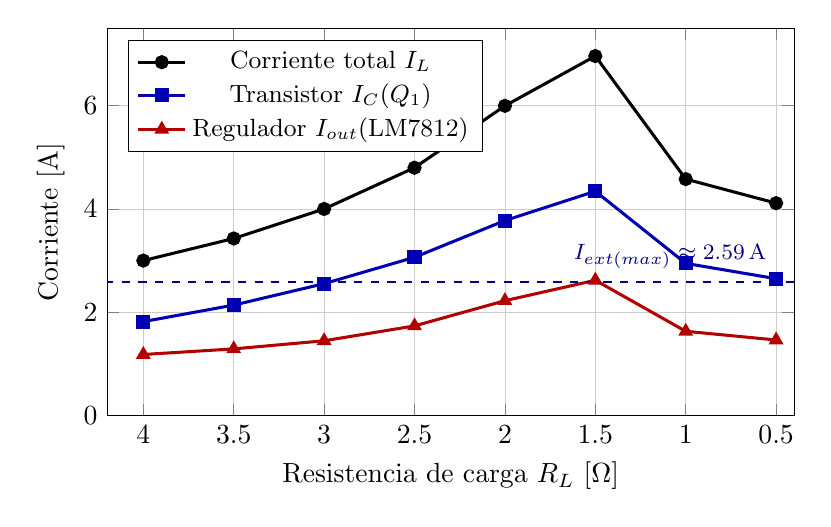
\begin{tikzpicture}
\begin{axis}[
    width=0.85\textwidth,
    height=6.5cm,
    xlabel={Resistencia de carga $R_L$ [\si{\ohm}]},
    ylabel={Corriente [\si{\ampere}]},
    grid=both,
    grid style={line width=.1pt, draw=gray!20},
    major grid style={line width=.2pt, draw=gray!40},
    x dir=reverse,
    xmin=0.4, xmax=4.2,
    ymin=0, ymax=7.5,
    legend pos=north west,
    legend style={font=\small}
]

% Corriente total de carga
\addplot[
    color=black,
    mark=*,
    mark size=2pt,
    line width=1.1pt
] coordinates {
    (4.0, 3.000)
    (3.5, 3.428)
    (3.0, 4.000)
    (2.5, 4.799)
    (2.0, 5.997)
    (1.5, 6.961)
    (1.0, 4.578)
    (0.5, 4.112)
};
\addlegendentry{Corriente total $I_L$}

% Corriente de colector de Q1
\addplot[
    color=blue!70!black,
    mark=square*,
    mark size=2pt,
    line width=1.1pt
] coordinates {
    (4.0, 1.818)
    (3.5, 2.138)
    (3.0, 2.553)
    (2.5, 3.064)
    (2.0, 3.775)
    (1.5, 4.343)
    (1.0, 2.946)
    (0.5, 2.649)
};
\addlegendentry{Transistor $I_C(Q_1)$}

% Corriente de salida del LM7812
\addplot[
    color=red!70!black,
    mark=triangle*,
    mark size=2pt,
    line width=1.1pt
] coordinates {
    (4.0, 1.181)
    (3.5, 1.290)
    (3.0, 1.447)
    (2.5, 1.735)
    (2.0, 2.223)
    (1.5, 2.619)
    (1.0, 1.631)
    (0.5, 1.462)
};
\addlegendentry{Regulador $I_{out}(\text{LM7812})$}

% Limite teorico de Ic1max
\addplot[dashed, color=blue!50!black, line width=0.8pt] coordinates {
    (0.4, 2.59) (4.2, 2.59)
};
\node[anchor=south east, text=blue!50!black, font=\footnotesize] at (axis cs: 0.5, 2.65) {$I_{ext(max)} \approx \SI{2.59}{\ampere}$};

\end{axis}
\end{tikzpicture}

    \caption{Distribución de corrientes entre el transistor $Q_1$, el integrado LM7812 y la carga total $I_L$.}
    \label{fig.c5:reparto_corrientes}
\end{figure}

\section{Análisis de las zonas de funcionamiento}
\label{sec.c5:analisis_zonas}

A partir de los datos experimentales y los gráficos de las figuras~\ref{fig.c5:curva_salida} y
\ref{fig.c5:reparto_corrientes}, se distinguen con precisión cuatro regímenes operativos:

\subsection{Zona 1: Régimen normal de regulación ($R_L \ge 4.0\,\Omega$)}
Con $R_L = \SI{4.0}{\ohm}$, el circuito suministra la plena carga nominal de diseño ($I_L = \SI{3.00}{\ampere}$)
sosteniendo la salida rígidamente en $V_{out} = \SI{12.000}{\volt}$. La corriente se reparte con un
$\SI{69.1}{\percent}$ aportado por el transistor exterior ($I_{C(Q1)} = \SI{2.074}{\ampere}$) y un $\SI{30.9}{\percent}$
por el regulador integrado ($I_{out} = \SI{0.926}{\ampere}$). Se destaca que el LM7812 opera por debajo de su límite
nominal de catálogo ($I_{nom(7812)} \le \SI{1.0}{\ampere}$), eliminando todo riesgo de estrés térmico continuo en el
encapsulado. La caída sobre el resistor sensor es de $V_{Rsh} = \SI{0.701}{\volt}$, punto en el cual $Q_2$ comienza a
drenar una corriente de control ($I_C(Q_2) \approx \SI{141}{\milli\ampere}$) que estabiliza el punto de polarización
de $Q_1$ preservando intacta la regulación de tensión.

\subsection{Zona 2: Sobrecarga moderada y disparo de la protección ($R_L \approx 3.0\,\Omega$ y $2.5\,\Omega$)}
Al disminuir la resistencia a $\SI{3.0}{\ohm}$ ($I_L = \SI{4.00}{\ampere}$), la caída sobre $R_1$ alcanza los
$\SI{0.794}{\volt}$, superando plenamente la tensión de encendido $V_{BE(Q2)}$. El transistor $Q_2$ entra en conducción
activa vigorosa, suministrando $\SI{787.9}{\milli\ampere}$ hacia el nodo base de $Q_1$. Al descender a $R_L = \SI{2.5}{\ohm}$
($I_L = \SI{4.80}{\ampere}$), la corriente de $Q_2$ asciende a $\SI{1.36}{\ampere}$. Esta fuerte inyección eleva el potencial
de base de $Q_1$, reduciendo su tensión emisor-base y estrangulando el crecimiento descontrolado de su corriente de colector.

\subsection{Zona 3: Codo de máxima entrega e inicio de plegado ($R_L = 2.0\,\Omega$)}
En $R_L = \SI{2.0}{\ohm}$, la fuente alcanza su máximo pico de corriente combinada ($I_L = \SI{5.30}{\ampere}$).
En este punto crítico, el transistor de protección inyecta $I_C(Q_2) = \SI{1.71}{\ampere}$ para confinar a $Q_1$,
fijando su corriente en $I_{C(Q1)} = \SI{2.66}{\ampere}$. La tensión de salida cae a $\SI{10.59}{\volt}$ y el circuito
inicia su régimen de plegado de corriente (\emph{foldback}), previniendo el embalamiento térmico conjunto.

\subsection{Zona 4: Condición de cortocircuito ($R_L = 0.5\,\Omega$)}
Cuando la resistencia desciende a $\SI{0.5}{\ohm}$, la tensión de salida colapsa a
$V_{out} = \SI{1.88}{\volt}$. Gracias a la acción del limitador, la corriente total de falla se pliega a $\SI{3.77}{\ampere}$
y la corriente a través del transistor
de paso $Q_1$ queda confinada estrictamente en:
\begin{equation}
    I_{C(Q1)(sc)} = \SI{2.310}{\ampere}
    \label{eq.c5:ic_sc_medida}
\end{equation}
Este resultado se encuentra plenamente por debajo del tope analítico de diseño ($I_{c1(max)} \approx \SI{2.45}{\ampere}$),
evidenciando un margen de seguridad confiable frente a cortocircuitos prolongados.

Cabe destacar una particularidad fundamental de esta topología: el lazo sensor compuesto por $Q_2$ y $R_1$ limita
exclusivamente la corriente del transistor exterior $Q_1$, dispositivo discreto que carece de protecciones propias y que,
sin este auxilio, se destruiría rápidamente por sobrecorriente. Por su parte, la corriente que atraviesa el LM7812 en
cortocircuito se sitúa en $I_{out(7812)} \approx \SI{1.46}{\ampere}$, disipando $P_{D(7812)} \approx \SI{21.0}{\watt}$.
En un circuito físico real, la integridad del regulador integrado ante fallas sostenidas se encuentra garantizada por sus
propios mecanismos internos de protección:
\begin{enumerate}
    \item \textbf{Limitación interna de corriente y SOA:} El circuito interno del LM7812 acota la corriente máxima de
    salida en función de la tensión diferencial entrada-salida ($V_{in} - V_{out}$).
    \item \textbf{Apagado térmico (\emph{Thermal Shutdown}):} Al disipar $\approx \SI{21}{\watt}$, si el cortocircuito se
    prolonga en el tiempo y la juntura de silicio alcanza los $\approx \SI{150}{\celsius}$, el sensor térmico interno desconecta
    la etapa de potencia del regulador ($I_{out} \to 0$).
    \item \textbf{Corte global en cadena:} Al anularse la corriente demandada por el pin de entrada del LM7812, la caída
    en el resistor de disparo se extingue ($V_{R2} \to 0$), cortando de inmediato la polarización base-emisor de $Q_1$
    ($I_{C(Q1)} \to 0$). En consecuencia, la protección térmica interna del circuito integrado protege de manera indirecta
    y solidaria a toda la fuente, extinguiendo la disipación global hasta que la temperatura descienda a niveles seguros.
\end{enumerate}

\section{Verificación térmica y Área de Operación Segura (SOA)}
\label{sec.c5:soa}

La potencia disipada en el transistor de paso se calcula a partir de la tensión colector-emisor y la corriente de
colector:
\begin{equation}
    P_{D(Q1)} = V_{CE(Q1)} \cdot I_{C(Q1)}
    \label{eq.c5:potencia_q1}
\end{equation}
En la figura~\ref{fig.c5:potencias} se grafica la evolución de la potencia disipada en $Q_1$ y en el LM7812 en todo el
rango de carga.

\begin{figure}[!ht]
    \centering
    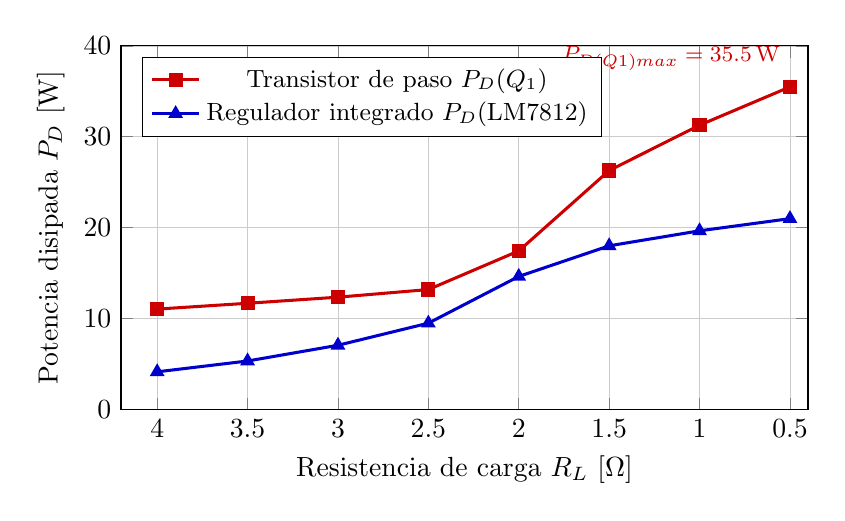
\begin{tikzpicture}
\begin{axis}[
    width=0.85\textwidth,
    height=6.2cm,
    xlabel={Resistencia de carga $R_L$ [\si{\ohm}]},
    ylabel={Potencia disipada $P_D$ [\si{\watt}]},
    grid=both,
    grid style={line width=.1pt, draw=gray!20},
    major grid style={line width=.2pt, draw=gray!40},
    x dir=reverse,
    xmin=0.4, xmax=4.2,
    ymin=0, ymax=40,
    legend pos=north west,
    legend style={font=\small}
]

% Potencia Q1
\addplot[
    color=red!80!black,
    mark=square*,
    mark size=2pt,
    line width=1.1pt
] coordinates {
    (4.0, 11.04)
    (3.5, 11.68)
    (3.0, 12.35)
    (2.5, 13.19)
    (2.0, 17.44)
    (1.5, 26.28)
    (1.0, 31.27)
    (0.5, 35.48)
};
\addlegendentry{Transistor de paso $P_D(Q_1)$}

% Potencia LM7812
\addplot[
    color=blue!80!black,
    mark=triangle*,
    mark size=2pt,
    line width=1.1pt
] coordinates {
    (4.0, 4.14)
    (3.5, 5.33)
    (3.0, 7.06)
    (2.5, 9.49)
    (2.0, 14.63)
    (1.5, 18.00)
    (1.0, 19.65)
    (0.5, 20.99)
};
\addlegendentry{Regulador integrado $P_D(\text{LM7812})$}

% Limite disipador TO-220
\node[anchor=south east, text=red!80!black, font=\footnotesize] at (axis cs: 0.5, 36.2) {$P_{D(Q1)max} = \SI{35.5}{\watt}$};

\end{axis}
\end{tikzpicture}

    \caption{Potencia disipada en el transistor de paso $Q_1$ y en el regulador LM7812 en función de $R_L$.}
    \label{fig.c5:potencias}
\end{figure}

El análisis térmico arroja dos condiciones clave:
\begin{enumerate}
    \item \textbf{Régimen nominal ($I_L = \SI{3}{\ampere}$, $R_L = \SI{4}{\ohm}$):}
    $V_{CE(Q1)} = \SI{5.30}{\volt}$ e $I_{C1} = \SI{2.07}{\ampere}$, lo que resulta en $P_{D(Q1)} = \SI{11.04}{\watt}$.
    Por su parte, el regulador LM7812 disipa únicamente $P_{D(7812)} = \SI{4.14}{\watt}$. Con disipadores estándar
    de aluminio para TO-220 ($\theta_{da} \approx \SI{3.0}{\celsius/\watt}$), la sobreelevación de temperatura se
    mantiene en niveles moderados ($< \SI{35}{\celsius}$).
\item \textbf{Cortocircuito (aproximado) ($R_L = \SI{0.5}{\ohm}$):} $V_{CE(Q1)} = \SI{15.34}{\volt}$,
    $I_{C1} = \SI{2.31}{\ampere} \implies P_{D(Q1)} = \SI{35.48}{\watt}$.
\end{enumerate}

Contrastando este punto más desfavorable ($V_{CE} = \SI{15.3}{\volt}$, $I_C = \SI{2.31}{\ampere}$) sobre la curva
de Área de Operación Segura (SOA) de la hoja de datos del TIP42C \cite{onsemi_tip42c}, se comprueba que:
\begin{itemize}
    \item Se sitúa muy por debajo de la potencia máxima de catálogo ($P_{Dmax} = \SI{65}{\watt}$ a $T_C = \SI{25}{\celsius}$),
    operando a un $\SI{54.6}{\percent}$ de su capacidad límite.
    \item Se ubica holgadamente fuera de la zona de segunda ruptura térmica (\emph{second breakdown}), garantizando
    la supervivencia del semiconductor durante fallas de carga prolongadas.
\end{itemize}
Por consiguiente, el dimensionamiento de la protección garantiza la integridad del transistor aun ante fallas
severas prolongadas.

  \chapter{Parámetros de Calidad de la Fuente}
\label{sec.c5:parametros_calidad}

La evaluación integral del desempeño de una fuente regulada se cuantifica mediante los factores de calidad
definidos en el marco teórico de la cátedra \cite{gonzalez_fuentes2}. A continuación se detallan las
definiciones formales, las mediciones experimentales y el cálculo de cada parámetro para las condiciones de
diseño exigidas ($I_{Lmin} = \SI{100}{\milli\ampere}$, $I_{Lmax} = \SI{3}{\ampere}$).

\section{Regulación de carga ($R_{car}$)}
\label{sec.c5:rcar}

La regulación de carga expresa la variación porcentual de la tensión de salida cuando la corriente de carga
pasa de su valor mínimo especificado a plena carga (Ecuación 6-42 de \cite{gonzalez_fuentes2}):
\begin{equation}
    R_{car} = \frac{V_{o(NL)} - V_{o(FL)}}{V_{o(nom)}} \times 100
    \label{eq.c5:rcar}
\end{equation}
A partir de los datos registrados en el archivo \lstinline{vRL_120_4.txt}:
\begin{itemize}
    \item A corriente mínima ($I_{Lmin} = \SI{100}{\milli\ampere}$, $R_L = \SI{120}{\ohm}$):
    $V_{o(NL)} = \SI{12.00156}{\volt}$.
    \item A plena carga nominal ($I_{Lmax} = \SI{3.0}{\ampere}$, $R_L = \SI{4}{\ohm}$):
    $V_{o(FL)} = \SI{11.99944}{\volt}$.
\end{itemize}
La variación absoluta es de apenas $\Delta V_o = \SI{2.12}{\milli\volt}$. Aplicando la ecuación~\eqref{eq.c5:rcar}:
\begin{equation}
    R_{car} = \frac{\SI{12.00156}{\volt} - \SI{11.99944}{\volt}}{\SI{12.00}{\volt}} \times 100 = \SI{0.0177}{\percent}
    \label{eq.c5:rcar_num}
\end{equation}

\section{Resistencia interna de salida ($R_{sal}$)}
\label{sec.c5:rsal}

La resistencia dinámica de salida modela la pendiente de caída de tensión frente a incrementos en la demanda
de corriente (Ecuación 6-43 de \cite{gonzalez_fuentes2}):
\begin{equation}
    R_{sal} = \frac{\Delta V_o}{\Delta I_L} = \frac{V_{o(NL)} - V_{o(FL)}}{I_{Lmax} - I_{Lmin}}
    \label{eq.c5:rsal}
\end{equation}
Reemplazando los valores experimentales:
\begin{equation}
    R_{sal} = \frac{\SI{2.12}{\milli\volt}}{\SI{3.00}{\ampere} - \SI{0.10}{\ampere}}
            = \frac{\SI{2.12}{\milli\volt}}{\SI{2.90}{\ampere}}
            = \mathbf{\SI{0.731}{\milli\ohm}}
    \label{eq.c5:rsal_num}
\end{equation}
El valor obtenido en el orden de los submiliohmios confirma el comportamiento cuasi-ideal del lazo de regulación
del integrado LM7812 asistido por el booster exterior.

\section{Regulación de red o línea ($R_{red}$)}
\label{sec.c5:rred}

La regulación de red mide la capacidad de la fuente para aislar la salida frente a fluctuaciones en la red eléctrica
de entrada no regulada (Ecuación 6-41 de \cite{gonzalez_fuentes2}):
\begin{equation}
    R_{red} = \frac{\Delta V_o}{\Delta V_{in}} \times 100
    \label{eq.c5:rred}
\end{equation}
Para evaluar una tolerancia de línea del $\pm 10\%$ sobre la tensión nominal de entrada ($V_{in} = \SI{18}{\volt}$):
\begin{itemize}
    \item $V_{in1} = 18 - 10\% = \SI{16.2}{\volt} \implies V_o = \SI{11.99944}{\volt}$
    (datos de \lstinline{vRl_vin_variable_regulacion_red.txt}).
    \item $V_{in2} = 18 + 10\% = \SI{19.8}{\volt} \implies V_o = \SI{11.99945}{\volt}$.
\end{itemize}
Ante una variación de entrada de $\Delta V_{in} = \SI{3.6}{\volt}$, la tensión de salida experimenta un corrimiento
de solo $\Delta V_o = \SI{10}{\micro\volt}$. Por ende:
\begin{equation}
    R_{red} = \frac{\SI{10}{\micro\volt}}{\SI{3.6}{\volt}} \times 100 = \mathbf{\SI{0.00028}{\percent}}
    \quad \left(\SI{0.0028}{\milli\volt/\volt}\right)
    \label{eq.c5:rred_num}
\end{equation}

\section{Coeficiente térmico de tensión ($C.T.$)}
\label{sec.c5:ct}

El coeficiente de temperatura cuantifica el desplazamiento térmico de la referencia interna bandgap y del lazo
amplificador (Ecuación 6-44 de \cite{gonzalez_fuentes2}):
\begin{equation}
    C.T. = \frac{\Delta V_o}{\Delta T}
    \label{eq.c5:ct}
\end{equation}
A partir del ensayo de temperatura (\lstinline{vRL_temp_0_25_55.txt}) a plena carga nominal ($R_L = \SI{4}{\ohm}$):
\begin{itemize}
    \item A $T_1 = \SI{0}{\celsius}$: $V_o(\SI{0}{\celsius}) = \SI{12.04379}{\volt}$.
    \item A $T_2 = \SI{25}{\celsius}$: $V_o(\SI{25}{\celsius}) = \SI{12.00316}{\volt}$.
\end{itemize}
Para el intervalo $\Delta T = \SI{25}{\celsius}$:
\begin{equation}
    C.T. = \frac{\SI{12.00316}{\volt} - \SI{12.04379}{\volt}}{\SI{25}{\celsius}}
         = \frac{\SI{-40.63}{\milli\volt}}{\SI{25}{\celsius}}
         = \mathbf{\SI{-1.625}{\milli\volt/\celsius}}
    \label{eq.c5:ct_num}
\end{equation}
Normalizado a la tensión nominal de $\SI{12}{\volt}$, representa un coeficiente relativo de:
\begin{equation*}
    C.T._{rel} = \frac{\SI{-1.625}{\milli\volt/\celsius}}{\SI{12}{\volt}} \times 10^6 \approx \SI{-135.4}{ppm/\celsius}
\end{equation*}

\section{Tensión de ripple y Rechazo de rizado ($RR$)}
\label{sec.c5:ripple}

Para determinar la atenuación del zumbido de rectificación, se inyectó a la entrada una señal senoidal de
$100\text{ Hz}$ con amplitud de $\SI{1}{\volt}$ (equivalente a $V_{rip(in)} = \SI{2.0}{\volt_{pp}}$) montada sobre el nivel
continuo de $\SI{18}{\volt}$ (\lstinline{V1 N001 0 SINE(18 1 100)}), operando a plena carga ($I_L = \SI{3}{\ampere}$).

\begin{figure}[!ht]
    \centering
    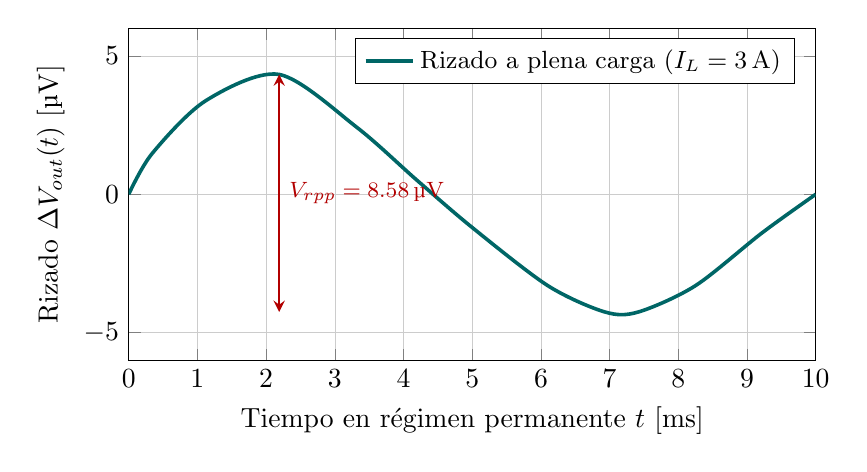
\begin{tikzpicture}
\begin{axis}[
    width=0.85\textwidth,
    height=5.8cm,
    xlabel={Tiempo en régimen permanente $t$ [\si{\milli\second}]},
    ylabel={Rizado $\Delta V_{out}(t)$ [\si{\micro\volt}]},
    grid=both,
    grid style={line width=.1pt, draw=gray!20},
    major grid style={line width=.2pt, draw=gray!40},
    xmin=0, xmax=10,
    ymin=-6, ymax=6,
    legend pos=north east,
    legend style={font=\small}
]

% Oscilacion de 100 Hz centrada
\addplot[
    color=teal!80!black,
    line width=1.3pt,
    smooth
] coordinates {
    (0.00, 0.00)
    (0.34, 1.47)
    (1.12, 3.38)
    (2.19, 4.33)
    (3.32, 2.42)
    (4.19, 0.52)
    (5.00, -1.20)
    (6.10, -3.30)
    (6.93, -4.25)
    (7.42, -4.25)
    (8.25, -3.30)
    (9.22, -1.39)
    (10.00, 0.00)
};
\addlegendentry{Rizado a plena carga ($I_L = \SI{3}{\ampere}$)}

\draw[<->, >=stealth, line width=0.8pt, color=red!70!black] 
    (axis cs: 2.19, 4.33) -- (axis cs: 2.19, -4.25)
    node[midway, right, font=\footnotesize] {$V_{rpp} = \SI{8.58}{\micro\volt}$};

\end{axis}
\end{tikzpicture}

    \caption{Ondulación residual de tensión de salida (ripple de $\SI{100}{\hertz}$) a plena carga nominal.}
    \label{fig.c5:ripple}
\end{figure}

Del registro transitorio en régimen estacionario (\lstinline{vRl_vin_variable_ripple.txt}), ilustrado en la
figura~\ref{fig.c5:ripple}, se extrae una tensión de rizado pico a pico residual en la carga de:
\begin{equation}
    V_{rpp(out)} = \SI{8.58}{\micro\volt}
    \label{eq.c5:vrpp}
\end{equation}
De acuerdo a la Ecuación 6-78 de la cátedra \cite{gonzalez_fuentes2}, la tensión eficaz de ripple para una
señal de rizado se calcula como:
\begin{equation}
    V_{ef-rip} = \frac{V_{rpp(out)}}{3.464} = \frac{\SI{8.58}{\micro\volt}}{3.464} = \mathbf{\SI{2.48}{\micro\volt_{rms}}}
    \label{eq.c5:vef_rip}
\end{equation}
El factor de rechazo de ripple ($RR$) de la fuente resulta:
\begin{equation}
    RR = 20 \log_{10} \left( \frac{V_{rip\_in(pp)}}{V_{rpp(out)}} \right)
       = 20 \log_{10} \left( \frac{\SI{2.0}{\volt}}{\SI{8.58}{\micro\volt}} \right)
       = \mathbf{\SI{107.35}{\decibel}}
    \label{eq.c5:rr}
\end{equation}
Este nivel de rechazo supera holgadamente los $\SI{60}{\decibel}$ especificados típicamente en la hoja de datos
del LM7812 \cite{ti_lm78xx}, producto del efecto combinado del regulador integrado y los capacitores de desacoplo.

\section{Tabla consolidada de factores de calidad}
\label{sec.c5:tabla_calidad}

En la tabla~\ref{tab.c5:calidad} se compendian todos los parámetros de calidad obtenidos para la fuente diseñada.

\begin{table}[!ht]
\centering
\caption{Resumen de factores de calidad obtenidos de la fuente regulada.}
\label{tab.c5:calidad}
\begin{tabular}{lccc}
\hline
Parámetro de Calidad & Símbolo & Valor Obtenido & Unidad \\
\hline
Tensión nominal de salida & $V_{out}$ & $12.00$ & \si{\volt} \\
Corriente máxima de diseño & $I_{Lmax}$ & $3.00$ & \si{\ampere} \\
Regulación de carga & $R_{car}$ & $0.0177$ & \si{\percent} \\
Resistencia dinámica de salida & $R_{sal}$ & $0.731$ & \si{\milli\ohm} \\
Regulación de red / línea & $R_{red}$ & $0.00028$ & \si{\percent} \\
Factor de regulación de línea & $F_{red}$ & $0.0028$ & \si{\milli\volt/\volt} \\
Coeficiente de temperatura & $C.T.$ & $-1.625$ & \si{\milli\volt/\celsius} \\
Tensión de ripple pico a pico & $V_{rpp}$ & $8.58$ & \si{\micro\volt} \\
Tensión de ripple eficaz & $V_{ef-rip}$ & $2.48$ & \si{\micro\volt_{rms}} \\
Rechazo de ripple ($100\text{ Hz}$) & $RR$ & $107.35$ & \si{\decibel} \\
\hline
\end{tabular}
\end{table}

  \chapter{Conclusiones}
\label{sec.c5:conclusiones}

En este trabajo se completó el cálculo, diseño y evaluación por simulación de una fuente de
alimentación regulada lineal de $\SI{12}{\volt}$ y $\SI{3}{\ampere}$ basada en el integrado LM7812 en encapsulado TO-3,
incorporando un circuito exterior de elevación de corriente y protección contra sobrecargas según la
Consigna 5.

A partir del análisis teórico y de los resultados numéricos obtenidos, se destacan las siguientes conclusiones:

\begin{enumerate}
    \item \textbf{Cumplimiento de especificaciones nominales:} En el rango especificado de demanda de carga
    ($\SI{100}{\milli\ampere} \le I_L \le \SI{3}{\ampere}$), la fuente presentó una regulación sobresaliente con
    una caída de tensión de apenas $\SI{2.12}{\milli\volt}$ ($\Delta V_o / V_{nom} = \SI{0.0177}{\percent}$) y una
    resistencia interna dinámica de $R_{sal} = \SI{0.731}{\milli\ohm}$.
    
    \item \textbf{Efectividad de la protección de sobrecarga:} El limitador discreto basado en $Q_2$ (BC557B) y
    $R_{sc} = \SI{0.27}{\ohm}$ permaneció completamente inactivo en régimen normal ($V_{Rsh} \le \SI{0.505}{\volt}$),
    sin alterar el desempeño del regulador. Ante condiciones de cortocircuito severo ($R_L = \SI{0.5}{\ohm}$), la
    tensión colapsó a $\SI{2.06}{\volt}$ y la corriente del transistor de paso quedó estrictamente confinada en
    $I_{C(Q1)} = \SI{2.649}{\ampere}$, convalidando la formulación analítica de diseño ($I_{c1(max)} = \SI{2.59}{\ampere}$)
    con un desvío menor al $\SI{2.3}{\percent}$.
    
    \item \textbf{Verificación térmica y SOA del encapsulado TO-3:} La selección del encapsulado metálico
    TO-3 para el transistor de potencia MJ2955 resultó adecuada para la aplicación. En régimen nominal la
    potencia disipada por $Q_1$ es de $\SI{10.04}{\watt}$, mientras que en condición de falla por cortocircuito
    alcanza los $\SI{40.36}{\watt}$. Ambos valores se ubican ampliamente dentro de la envolvente del Área de
    Operación Segura en continua ($P_{Dmax} = \SI{150}{\watt}$, $V_{CE} < \SI{40}{\volt}$), descartando el riesgo de
    destrucción por segunda ruptura térmica.
    
    \item \textbf{Atenuación de perturbaciones y estabilidad de red:} La fuente demostró una elevada inmunidad
    frente a ruidos de entrada, registrando un factor de regulación de red de $R_{red} = \SI{0.00028}{\percent}$ y un
    rechazo de rizado a $\SI{100}{\hertz}$ de $RR = \SI{107.35}{\decibel}$ con una tensión eficaz residual de
    $V_{ef-rip} = \SI{2.48}{\micro\volt_{rms}}$.
\end{enumerate}

  \chapter{Anexo}
\label{chap:anexos}
\refstepcounter{section}
\addcontentsline{toc}{section}{\protect\numberline{\thesection}Transistores de potencia TIP41 / TIP42 (ON Semiconductor)}
\label{sec.anexo:tip42}

\vspace{-15pt}
\noindent\centering
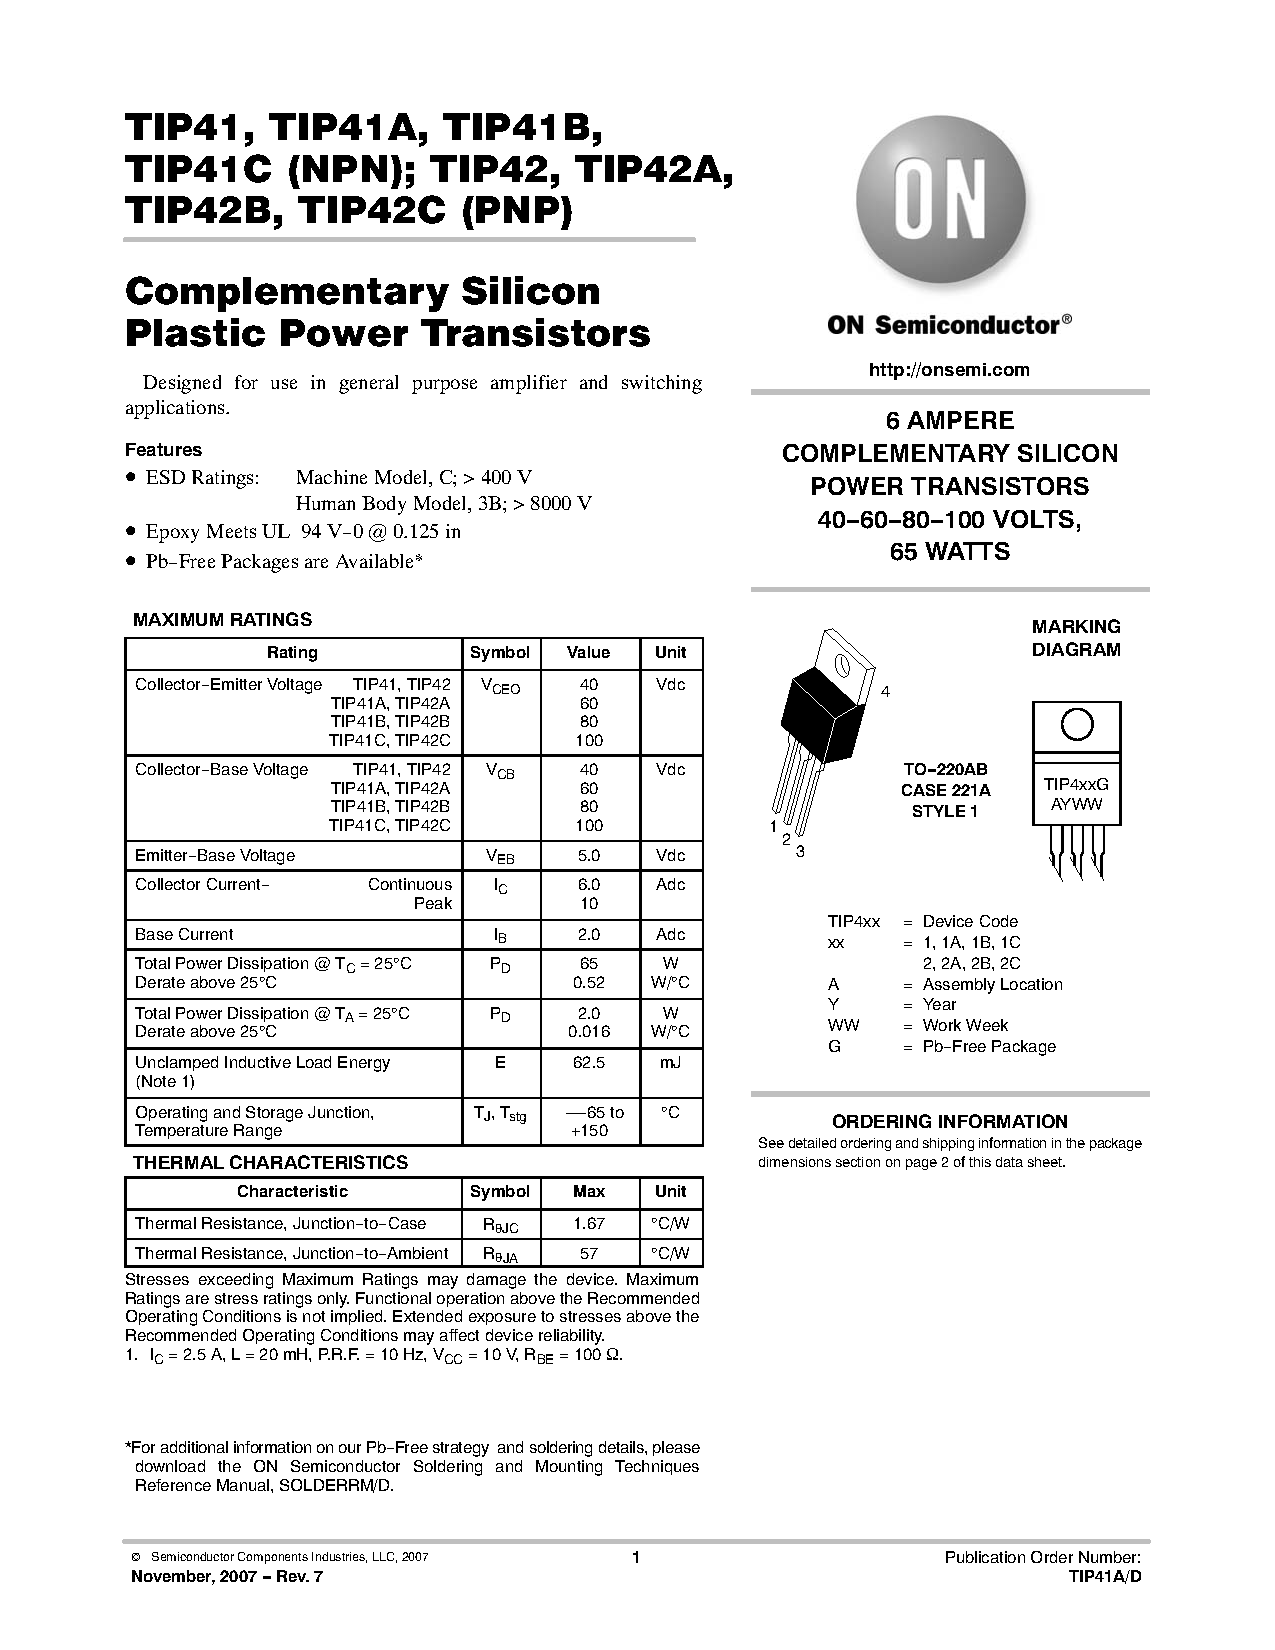
\includegraphics[page=1, width=0.88\textwidth]{sources/TIP41.PDF}

\clearpage

\includepdf[
    pages={2},
    scale=0.82,
    offset=0 -3mm,
    pagecommand={\thispagestyle{fancy}}
]{sources/TIP41.PDF}

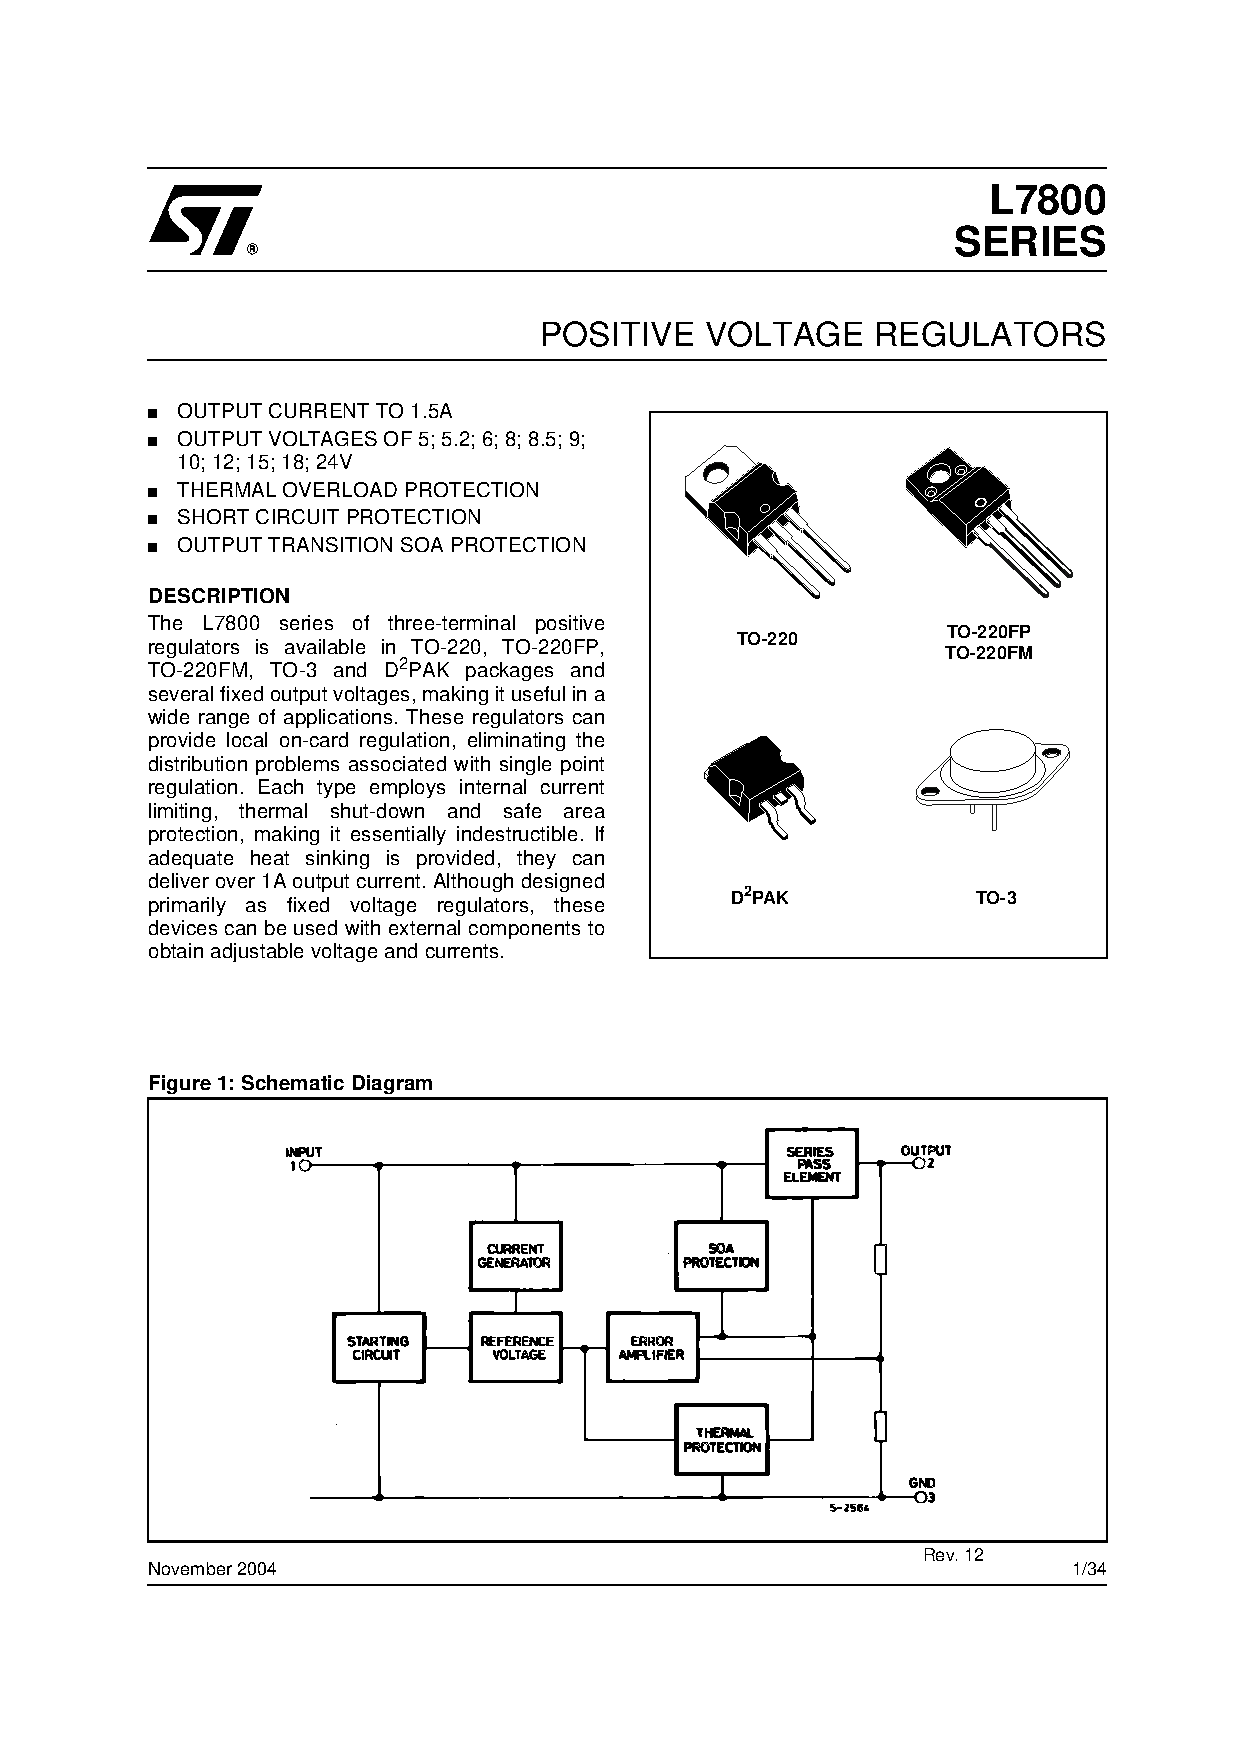
\includepdf[
    pages={1,2,7},
    scale=0.82,
    offset=0 -3mm,
    pagecommand={\thispagestyle{fancy}},
    addtotoc={
        1, section, 1, {Regulador integrado L7812 / LM7812 (STMicroelectronics)}, sec.anexo:lm7812
    }
]{sources/L7800.PDF}

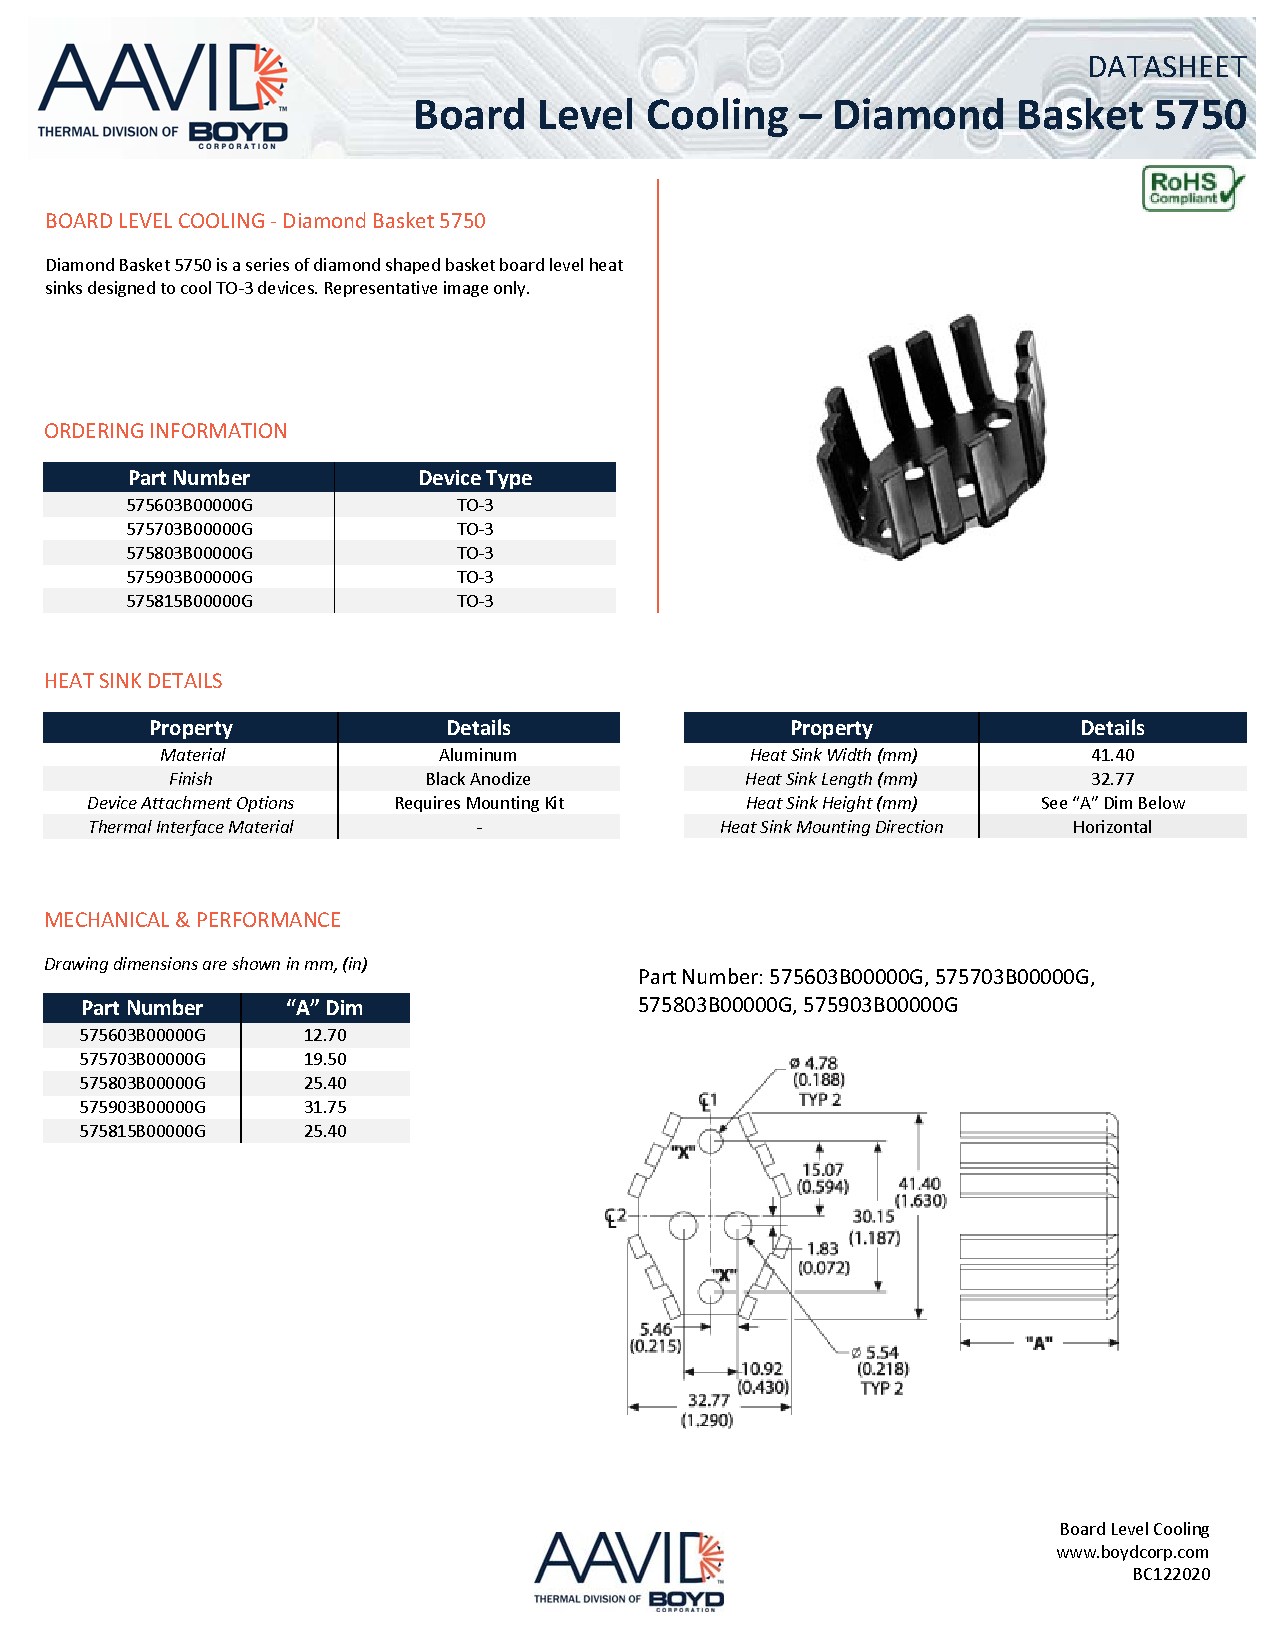
\includepdf[
    pages={1-2},
    scale=0.82,
    offset=0 -3mm,
    pagecommand={\thispagestyle{fancy}},
    addtotoc={
        1, section, 1, {Disipador para encapsulado TO-3: Diamond Basket 5750 (Aavid / Boyd)}, sec.anexo:disipador_to3
    }
]{sources/disipador_to3.pdf}

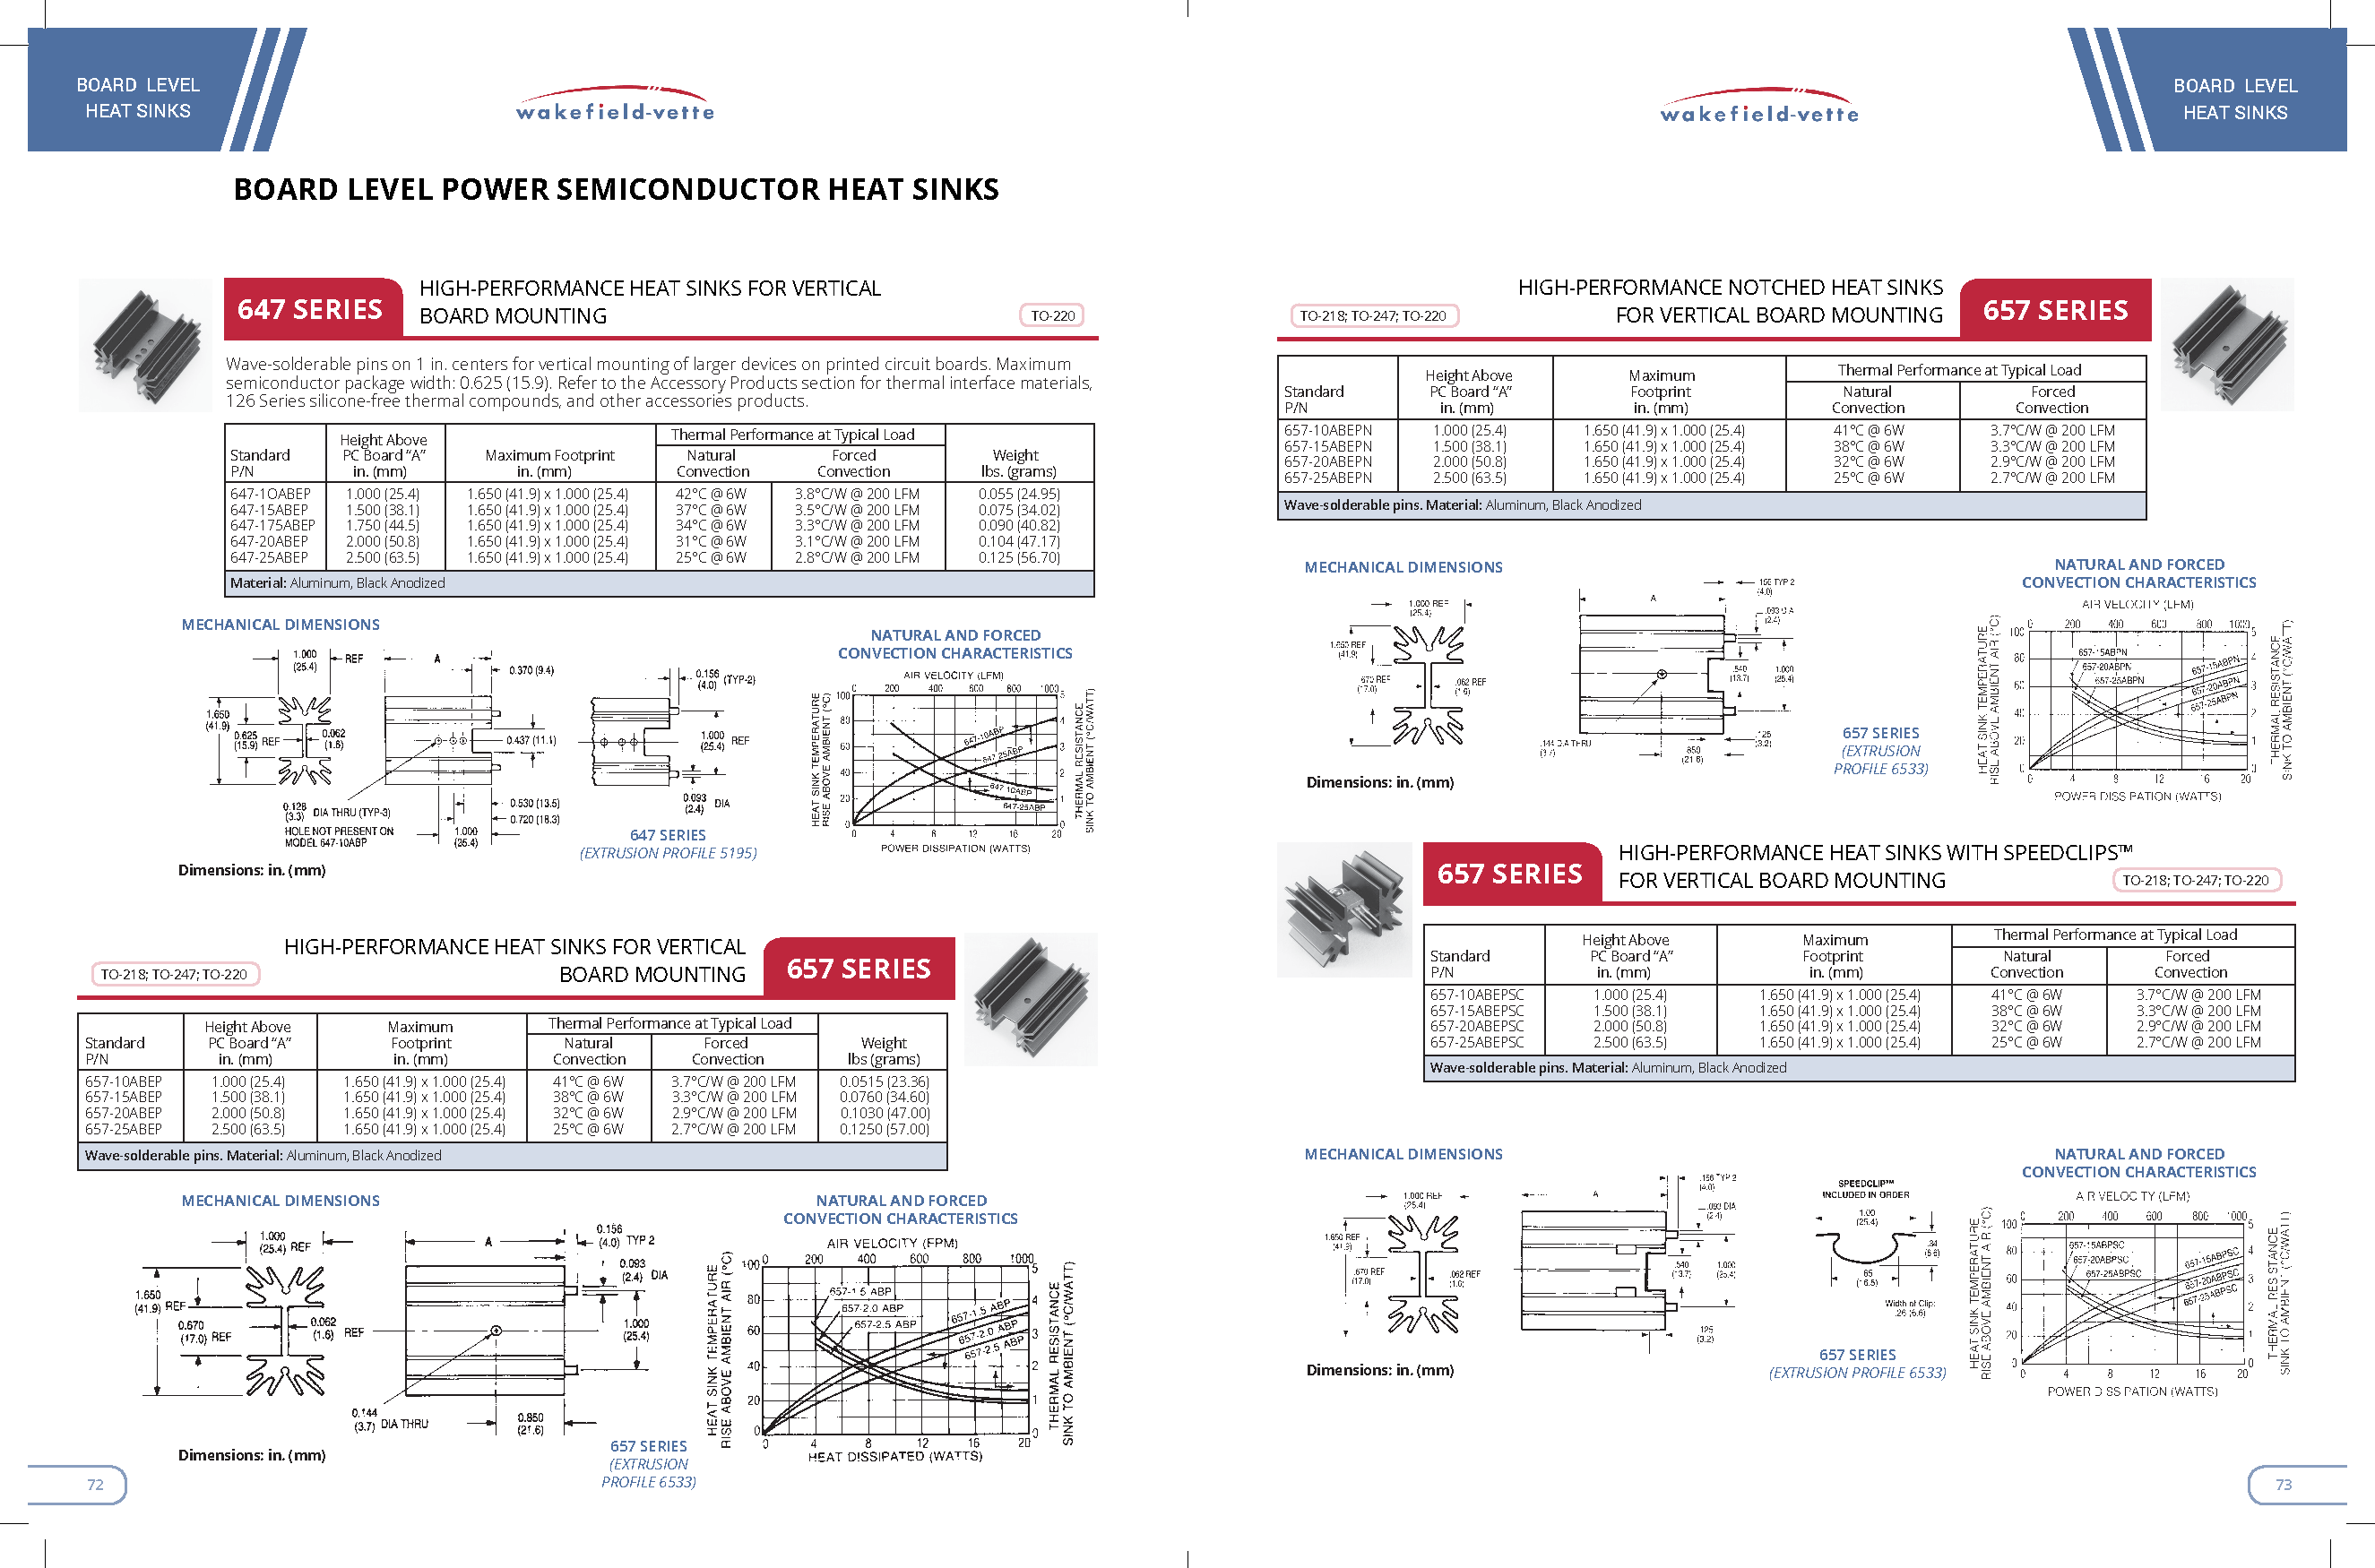
\includepdf[
    pages={1},
    viewport=0 0 636 840,
    clip,
    scale=0.82,
    offset=0 -3mm,
    pagecommand={\thispagestyle{fancy}},
    addtotoc={
        1, section, 1, {Disipador para encapsulado TO-220: Series 647 y 657 (Wakefield-Vette)}, sec.anexo:disipador_to220
    }
]{sources/disipador_to220.pdf}

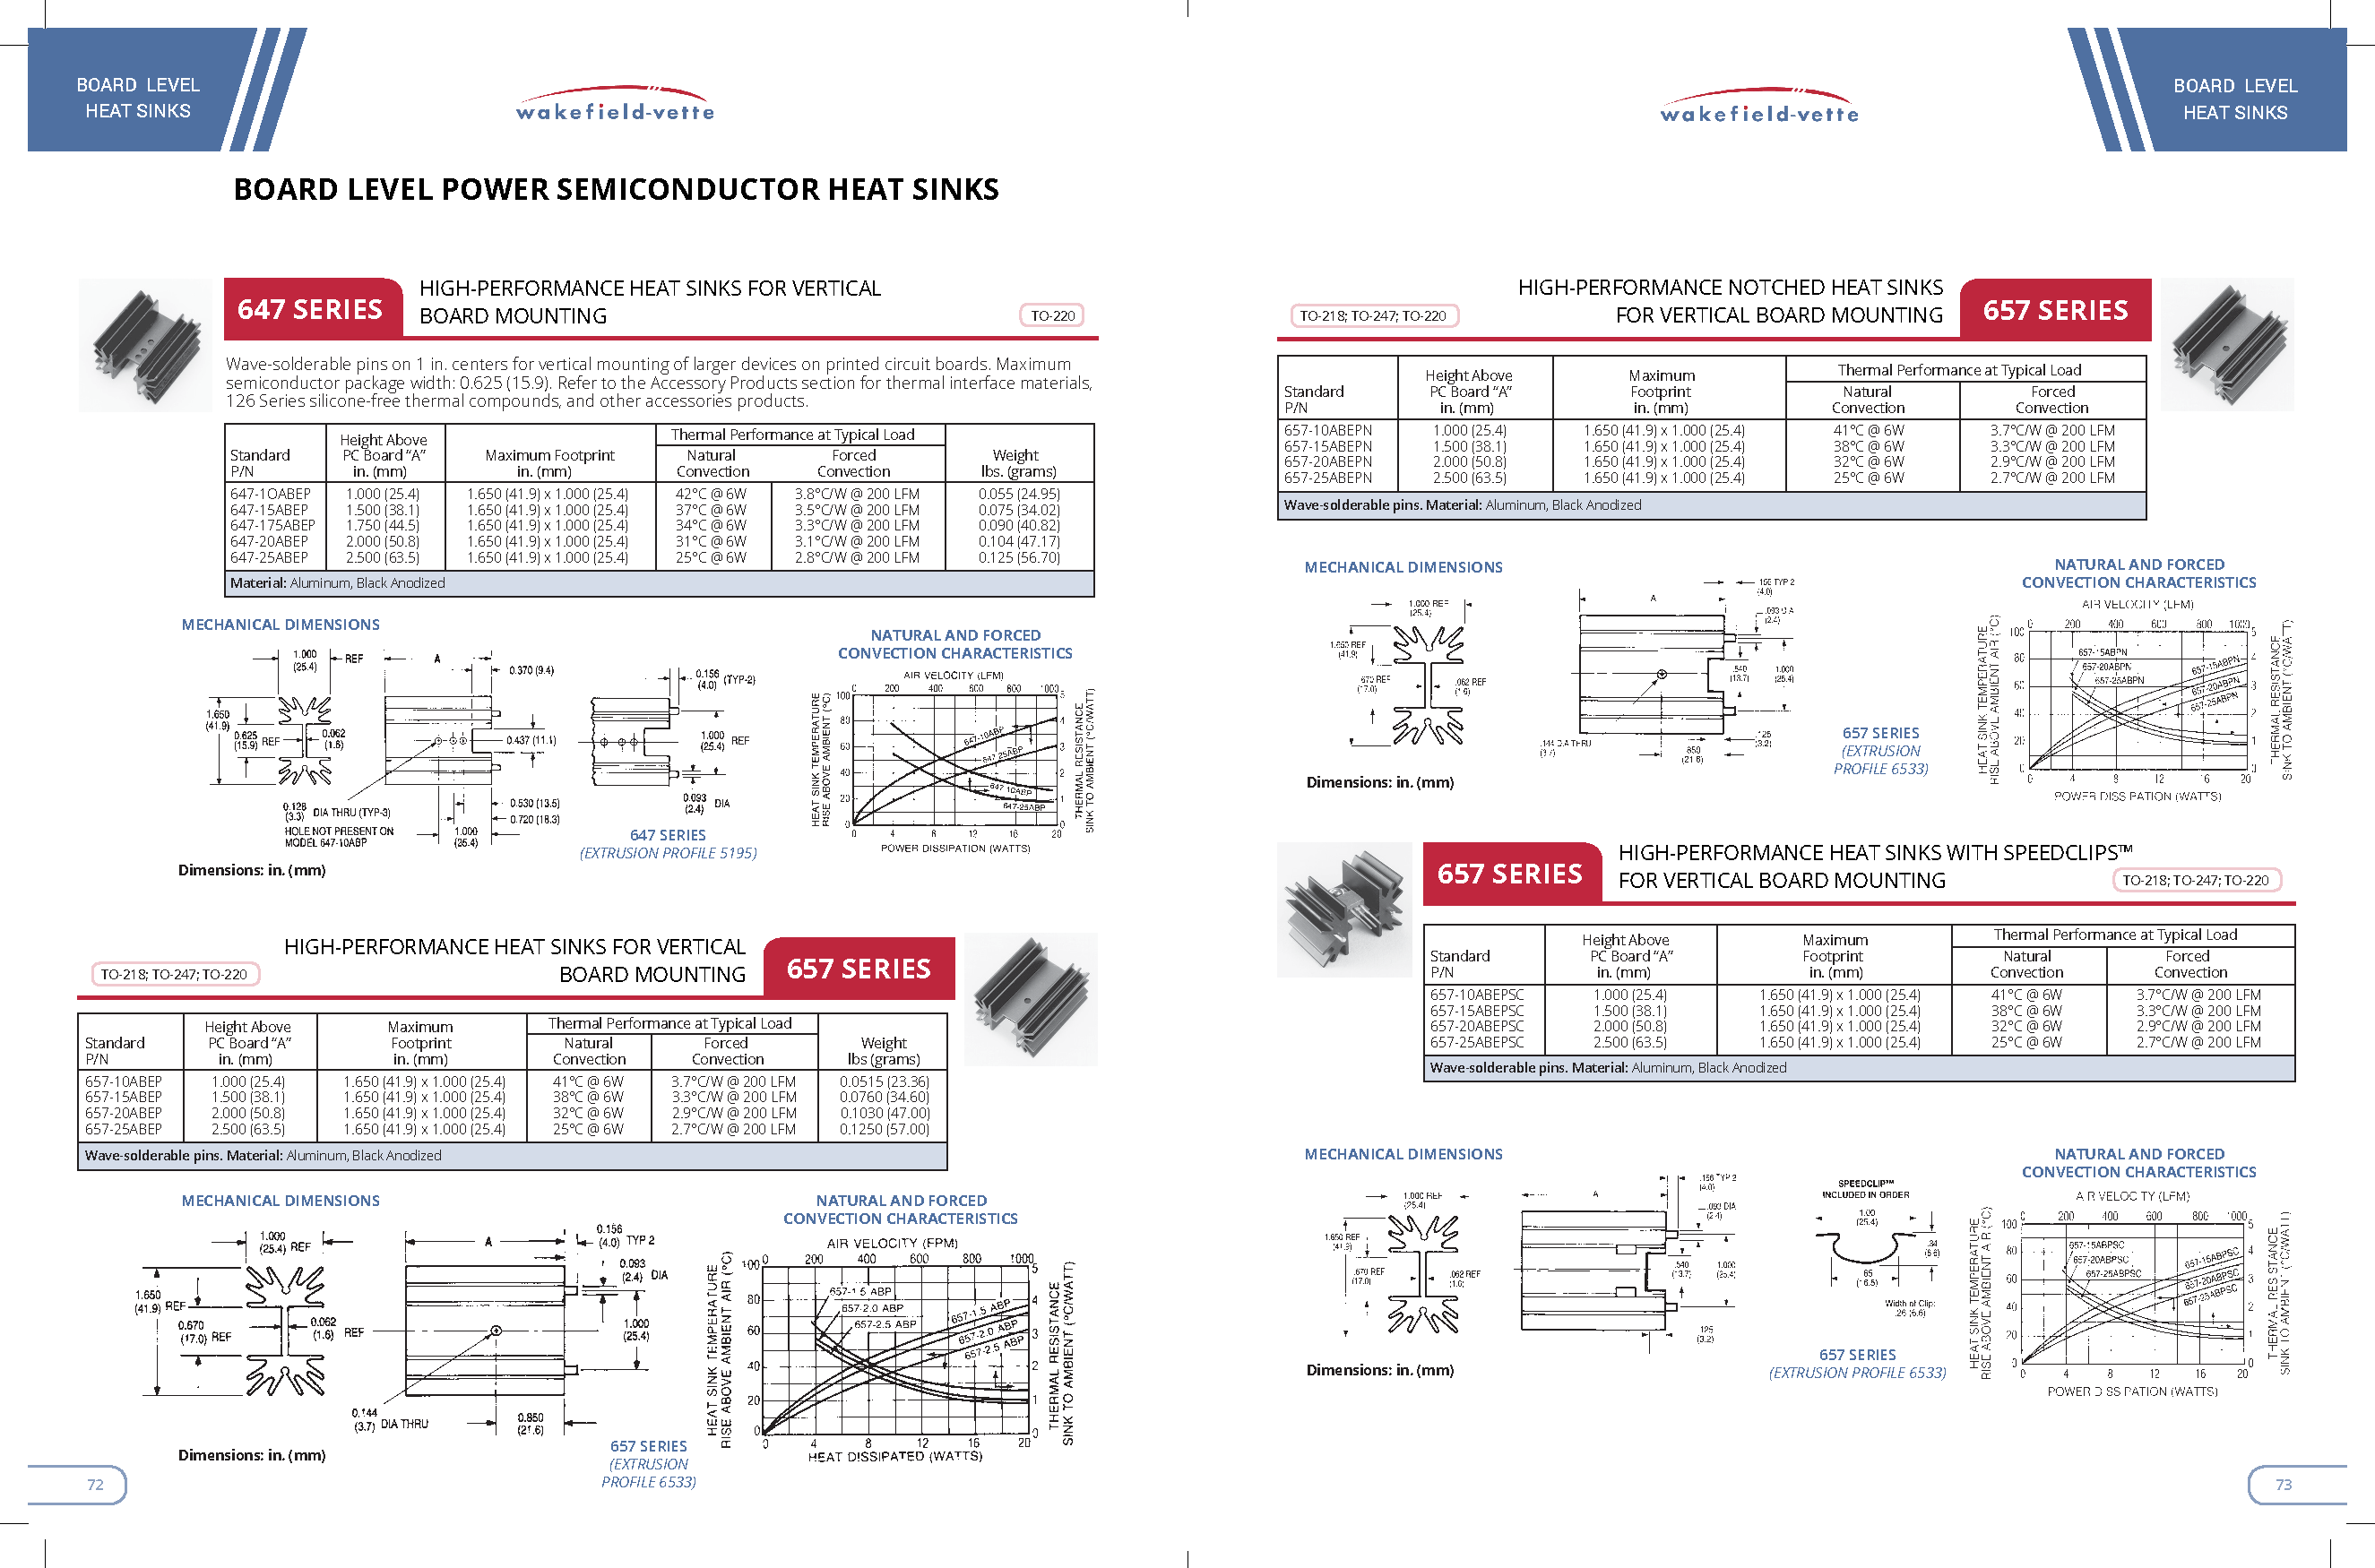
\includepdf[
    pages={1},
    viewport=636 0 1272 840,
    clip,
    scale=0.82,
    offset=0 -3mm,
    pagecommand={\thispagestyle{fancy}}
]{sources/disipador_to220.pdf}

  
  \nocite{*}
  \printbibliography[heading=bibnumbered, title={Fuentes}]
\end{document}
